\section{实验与结果分析}
在本章节中,我们评估了~\Mname{}在各种GNN模型和图数据集上的性能,对~\Mname{}的加速效果进行了全面的分析,并与现有的GNN框架(如DGL和PyG)进行了比较。我们还进行了一些附加实验研究,对GNN的隐藏维度,~\Mname{}的参数选择等问题进行了探讨。
\subsection{实验设置}
\hspace{5pt} \textbf{基准测试 (Benchmarks): }
我们选择了先前工作~\cite{wang2019dgl,pyG,ma2019neugraph} 在节点分类任务中广泛使用的两个最具代表性的 GNN 模型,以覆盖不同类型的聚合操作。
\underline{1) 图卷积网络 (GCN)}~\cite{GCNConv} 是最流行的 GNN 模型架构之一。
它也是许多其他 GNN(如图采样网络 GraphSAGE~\cite{SageConv} 和可微分池化 Diffpool~\cite{diffpool})的关键骨干网络。因此,提升 GCN 的性能也将惠及广泛的 GNN 模型。对于 GCN 的评估,我们采用以下设置:\textit{2 个层,隐藏维度为 16},这也是原始论文~\cite{GCNConv} 中的设置。
\underline{2) 图同构网络 (GIN)}~\cite{GINConv}。
GIN 与 GCN 的不同之处在于其聚合函数,该函数对节点自身的嵌入值进行加权。此外,GIN 也是许多其他具有更多边属性的更高级 GNN(如图注意力网络 GAT~\cite{GATConv})的参考架构。对于 GIN 的评估,我们采用以下设置:\textit{5 个层,隐藏维度为 64},这是原始论文~\cite{GINConv} 中使用的设置。

\textbf{基线 (Baselines): }
我们选择了两种同样基于 Pytorch 的图神经网络框架作为基线进行比较。
\underline{1) {Deep Graph Library (DGL})}~\cite{wang2019dgl} DGL 是一个专注于 GNN 计算效率的框架,特别是在 GPU 加速方面。它提供了针对多种主流 GNN 架构的高度优化的内核实现,并在许多标准图数据集和任务上展现出强大的性能。DGL 通过其底层的张量操作优化和高效的图表示,致力于为用户提供易于使用且性能卓越的 GNN 开发体验。
\underline{2) {Pytorch-Geometric (PyG})}~\cite{pyG} PyG 是另一个极其流行且功能强大的 GNN 框架,同样构建于 PyTorch 之上。PyG 以其灵活性和易于扩展性而闻名,尤其是在定义自定义 GNN 层和消息传递机制方面。它提供了一套简洁的 API,方便研究人员快速实现和迭代新颖的 GNN 模型。PyG 同样在性能方面表现出色,并在各种研究和应用中被广泛采用。

\textbf{数据集 (Datasets): }
我们涵盖了先前 GNN 相关工作~\cite{wang2019dgl, pyG, ma2019neugraph} 中使用的所有三种类型的数据集。
\underline{I 型图}是先前 GNN 算法论文~\cite{GCNConv, GINConv, SageConv} 常用的典型数据集。
它们的节点和边数量通常较小,但节点嵌入信息丰富且维度较高。
% These graphs can validate pure algorithm performance (\textit{e.g.}, the accuracy of link prediction).
% % 这些图可以验证纯粹的算法性能(例如,链接预测的准确性)。
\underline{II 型图}~\cite{KKMMN2016} 是图核 (graph kernels) 的流行基准数据集,并被选为 PyG~\cite{pyG} 的内置数据集。每个数据集包含一组小图,这些小图仅有图内边连接,没有图间边连接。
% These graphs are generally used for batched training or inference.
% % 这些图通常用于批量训练或推理。
\underline{III 型图} ~\cite{snapnets, GCNConv} 在节点和边的数量都很大。这些图表现出高度的结构不规则性,这对大多数现有的 GNN 框架来说都具有挑战性。这些数据集的详细信息列于表~\ref{table: Evaluation Dataset}。
 % Note that $\#Class$ is used for node classification task.
其中,\textbf{\#类型}于节点分类任务。
\begin{table}[htbp] 
    \footnotesize % 使用较小的字体
    \caption{用于评估的数据集}
    \vspace{5pt} % 添加垂直空间,避免caption与表格重叠
    \centering
    \resizebox{0.9\textwidth}{!}{ % 使表格宽度与正文相同
        \begin{tabular}{|c|l|r|r|r|r|}
        \hline
        \textbf{类型} & \textbf{数据集} & \textbf{\#顶点} & \textbf{\#边} & \textbf{维度} & \textbf{\#类别} \\
        \hline
        \multirow{4}{*}{\textbf{I}} 
        & Citeseer    & 3,327	    & 9,464	    & 3,703 & 6      \\
        & Cora	    & 2,708     & 10,858	& 1,433 & 7      \\
        & Pubmed	    & 19,717	& 88,676	& 500  & 3      \\
        & PPI	        & 56,944	& 818,716	& 50   & 121    \\
        \hline
        
        \multirow{6}{*}{\textbf{II}}
        & PROTEINS\_full	&   43,471	       & 162,088	&   29	    & 2 \\
        & OVCAR-8H	    &   1,890,931	   & 3,946,402	&   66	    & 2 \\
        & Yeast	        &   1,714,644	   & 3,636,546	&   74	    & 2 \\
        & DD	            &   334,925	       & 1,686,092	&   89	    & 2 \\
        & TWITTER-Partial	&   580,768	       & 1,435,116	& 1,323    & 2 \\
        & SW-620H	        &   1,889,971	   & 3,944,206	&   66	    & 2 \\
        \hline
        
        \multirow{5}{*}{\textbf{III}} 
        & amazon0505	    & 410,236	& 4,878,875	    & 96  & 22 \\
        & artist	        & 50,515	& 1,638,396	    & 100 & 12 \\
        & com-amazon	    & 334,863	& 1,851,744	    & 96  & 22 \\
        & soc-BlogCatalog	& 88,784	& 2,093,195	    & 128 & 39 \\
        & amazon0601	    & 403,394	& 3,387,388	    & 96 & 22 \\
        \hline
        \end{tabular}
    }
    \vspace{-5pt}
    \label{table: Evaluation Dataset}
\end{table}


\textbf{平台与指标 (Platforms \& Metrics): }
\label{sect: Platforms and Metrics }
我们使用 CUDA 12.4 和 PyTorch 2.4.0 作为编程平台,基于 C++ 和 CUDA 实现了 ~\Mname{} 的后端,并通过 Python 绑定 PyTorch 前端。评估平台采用了一台配备 16 核心、32 线程的 AMD Ryzen 9 7945HX 处理器和 NVIDIA RTX 4060 GPU 的笔记本电脑,运行环境为 WSL2 下的 Ubuntu 24.04。在性能评估过程中,为了量化加速效果,我们通过计算 200 次端到端推理(前向传播)和训练(前向传播和反向传播)的平均延迟(不包括i数据预处理和加载时间)来衡量性能提升。
\begin{figure}[htbp] 
    \centering
    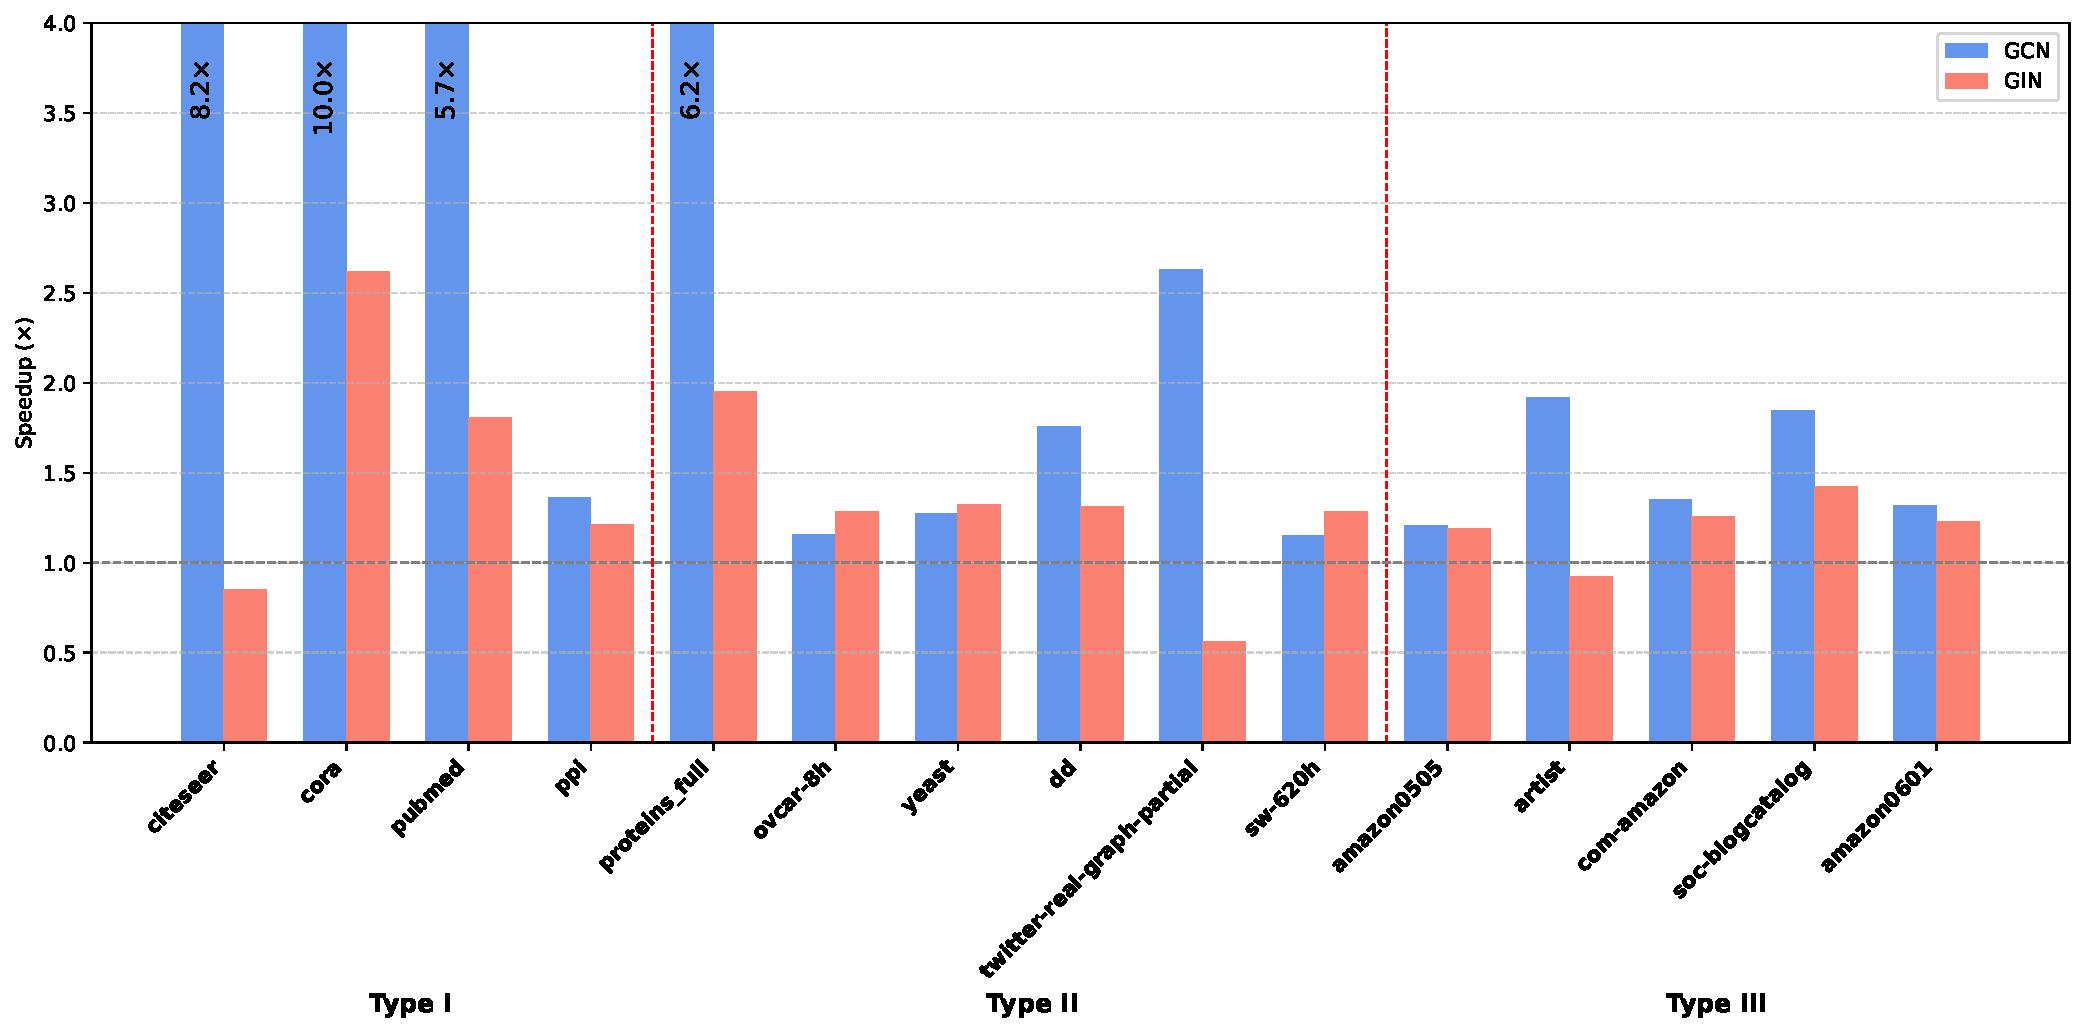
\includegraphics[width=0.9\linewidth]{images/dgl_infer_cmp.pdf} 
    \caption{~\Mname{} 在 GCN 和 GIN 上相较于 DGL 的推理加速比 ($\times$)。}
    \label{fig: Speedup vs DGL inference}
    \setlength{\abovecaptionskip}{0.4cm} %增大caption和图像之间的距离    
    \setlength{\belowcaptionskip}{-0.4cm} %缩小caption和下方文字的距离
\end{figure}
\subsection{性能评估}
在本节中,我们首先对比分析了~\Mname{}与 DGL 在图神经网络(GNN)推理任务中的性能差异,随后将对比扩展至训练任务。
如图~\ref{fig: Speedup vs DGL inference} 所示,~\Mname{}在 GCN 和 GIN 两类模型的推理任务中,分别在三类数据集上相较于 DGL~\cite{wang2019dgl} 平均加速达到了$3.13\times$ 和 、$1.35\times$。尤其是在挑战性较高的第三类图上,~\Mname{}对于 GCN 和 GIN 的平均加速分别为$1.53\times$ 和$1.12\times$。 这得益于~\Mname{}充分挖掘输入图的结构信息(如节点度数)用于指导系统优化。具体而言,我们基于节点分组策略进行工作负载划分,从而提升了 GPU 利用率。我们接下来将针对三类图数据展开具体分析,并探讨其中的性能优化机理。

\textbf{I 型图:}
对于该类图,GCN 相比 DGL 的加速效果明显优于 GIN,平均分别为$6.30\times$ 与$1.35\times$。
两者差异主要源自其各自的计算流程:GCN 在聚合操作之前进行节点特征降维(即 DGEMM 操作),显著减少了聚合阶段的数据移动和线程同步开销。这种结构非常契合 \Mname 所提出的二维任务划分机制和面向局部性的内存优化策略,能充分发挥 GPU 的数据局部性优势。
而 GIN 的计算顺序则相反,必须先执行聚合操作再进行节点特征变换,因此无法避免高频次的全局内存访问和数据传输,限制了数据局部性和共享内存的优势发挥。
尽管如此,我们提出的细粒度维度划分策略依然能够较好地处理高维特征场景,保障整体性能。

\textbf{II 型图:}
在这类图上,~\Mname{}依然取得了较为显著的性能提升,在 GCN 和 GIN 上平均加速比分别为$2.37\times$ 与$1.27\times$,但在 \textit{TWITTER-Partial} 数据集上差距略大,尤其是在 GIN 上,效果逊色于 DGL。该数据集的节点特征维度高达 1323,是此类图中最高的。而GIN 必须先在1323 维节点嵌入上执行邻居聚合,再进行线性变换降维。这导致了大量的全局内存访问和线程间同步开销,限制了性能提升。相比之下,GCN 先进行线性变换降维,再执行邻居聚合,因此在该数据集上仍然能够获得较好的加速效果。

\textbf{III 型图:}
这些图在节点和边的数量上都很大,表现出高度的结构不规则性,极具挑战性,但是~\Mname{}依然取得了一定效果。例如\textit{soc-BlogCatalog},~\Mname{} 对 GCN 和 GIN 的平均加速比分别达到$1.85\times$ 与$1.43\times$。这类图通常存在较高的线程间同步和全局内存访问开销,而我们提出的二维任务划分与内存优化机制可有效缓解这一瓶颈。此外,我们基于社区结构的信息进行的节点重新编号,进一步提升了线程之间在局部节点处理中的数据共享效率,从而提高了空间与时间局部性。但在 \textit{artist} 数据集上,GIN 的加速效果相对较低。分析发现,该数据集社区划分的标准差最高,社区结构分布极不均衡,导致我们难以充分利用社区信息在 GNN 聚合阶段捕捉局部性,也限制了线程映射对齐、共享内存调度等系统优化策略的实施效果。
\begin{figure}[htbp] 
    \centering
    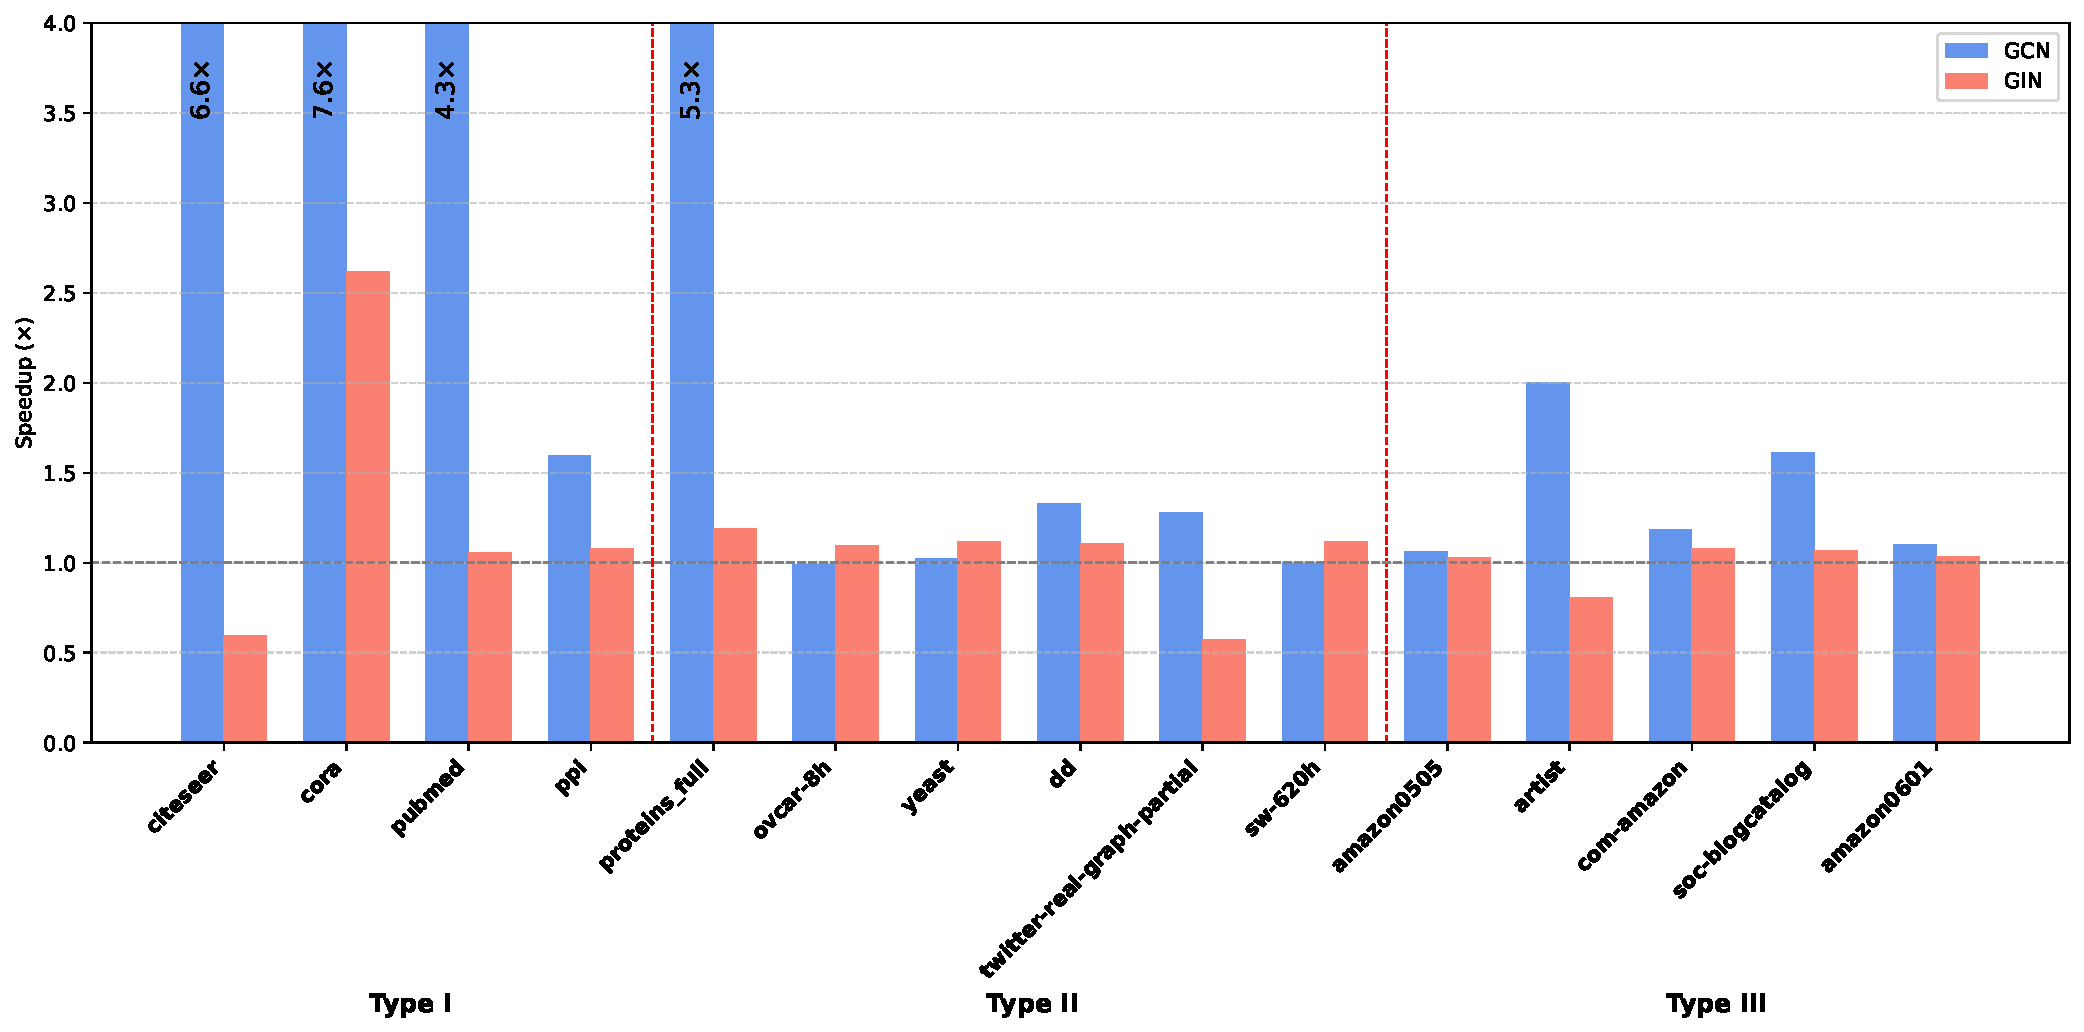
\includegraphics[width=0.9\linewidth]{images/dgl_train_cmp.pdf} 
    \caption{~\Mname{} 在 GCN 和 GIN 上相较于 DGL 的训练加速比 ($\times$)。}
    \label{fig: Speedup vs DGL Training}
    \setlength{\abovecaptionskip}{0.4cm} %增大caption和图像之间的距离    
    \setlength{\belowcaptionskip}{-0.4cm} %缩小caption和下方文字的距离
\end{figure}

\textbf{训练性能评估:}
我们进一步评估了 ~\Mname{} 在 GCN 和 GIN 模型上的训练性能,并与 DGL 进行了对比。
相比推理,训练过程更加复杂,涉及前向传播与反向传播两个阶段,二者均严重依赖底层图聚合计算的性能。如图~\ref{fig: Speedup vs DGL Training}所示,~\Mname{} 在 GCN 和 GIN 上的平均训练加速比分别为$1.61\times$ 和$2.00\times$,验证了我们基于输入特性优化策略的普适性与有效性。训练与推理的主要差异体现在两个方面:首先,训练过程中需要执行反向传播,这一阶段与推理中的前向计算类似,因此仍能从我们提出的优化中获益;其次,训练中需额外存储前向过程中的中间结果,直到反向传播使用,这会引入额外的数据访问与内存占用开销。因此,训练阶段的整体加速比相对推理阶段略低,这是由其本质的资源需求所决定的。
\begin{figure}[htbp] 
    \centering
    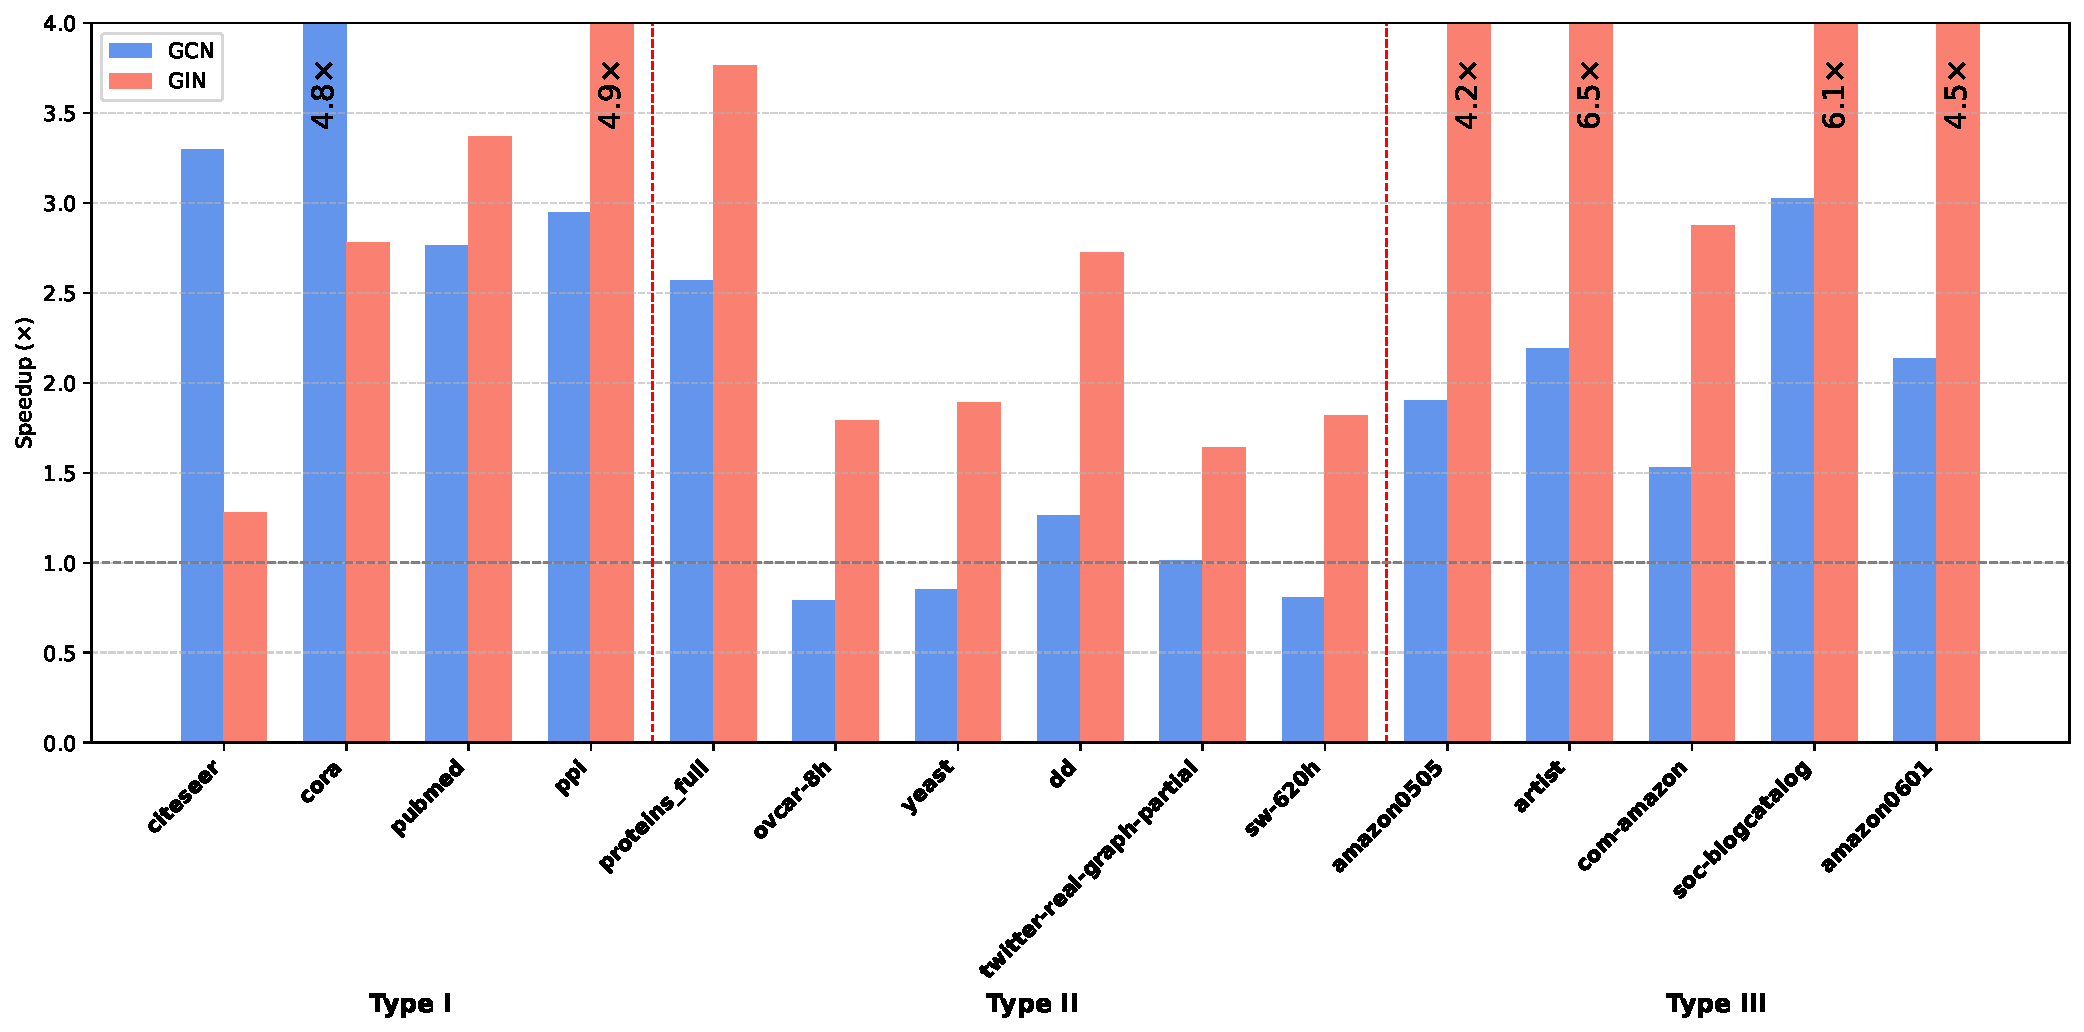
\includegraphics[width=0.9\linewidth]{images/pyg_infer_cmp.pdf} 
    \caption{~\Mname{} 在 GCN 和 GIN 上相较于 PyG 的推理加速比 ($\times$)。}
    \label{fig: Speedup vs PyG inference}
    \setlength{\abovecaptionskip}{0.4cm} %增大caption和图像之间的距离    
    \setlength{\belowcaptionskip}{-0.4cm} %缩小caption和下方文字的距离
\end{figure}
\subsubsection{和PyG的比较}
相比于 PyG,\Mname{} 展现出显著的性能优势。在 GCN 和 GIN 模型上,\Mname{} 的训练速度分别提升了 $2.13\times$ 和 $3.34\times$,推理速度则提升了 $3.13\times$ 和 $1.35\times$。其中,在 I 型图与 III 型图数据集上表现尤为突出,具体原因已在与 DGL 的对比分析中详细探讨,此处不再赘述。以下重点分析 ~\Mname{} 在 II 型图上的表现差异。

在 II 型图数据集上,~\Mname{} 的性能优势不明显,甚至在某些情况下表现不佳。以 GCN 为例,除 \textit{Proteins\_full} 数据集外,其余数据集的平均训练加速比$0.92\times$,平均推理加速比$0.94\times$,未能超过 PyG。这是因为PyG针对此类具有分块对角化邻接矩阵特性的批处理图数据优化最为全面(例如小批量处理机制),能够高效处理此类图结构数据。相比之下,~\Mname{} 仍然沿用了以节点度为基础的任务划分策略,在图规模较小、结构较为稠密的 II 型图中未能充分利用硬件资源,导致性能受限。

值得注意的是,在 GIN 模型上,\Mname{} 即便在 II 型图上仍取得了良好效果,实现了 $1.95\times$ 的训练加速和 $2.67\times$ 的推理加速。这主要归因于 GIN 所引入的线性变换操作在特征聚合阶段引入了更重的计算负载,~\Mname{} 的维度工作线程划分策略和线程束级线程对齐策略能够更好地适应这一计算模式,充分利用 GPU 的计算资源和内存带宽,从而实现了更高的性能提升。
\begin{figure}[htbp] 
    \centering
    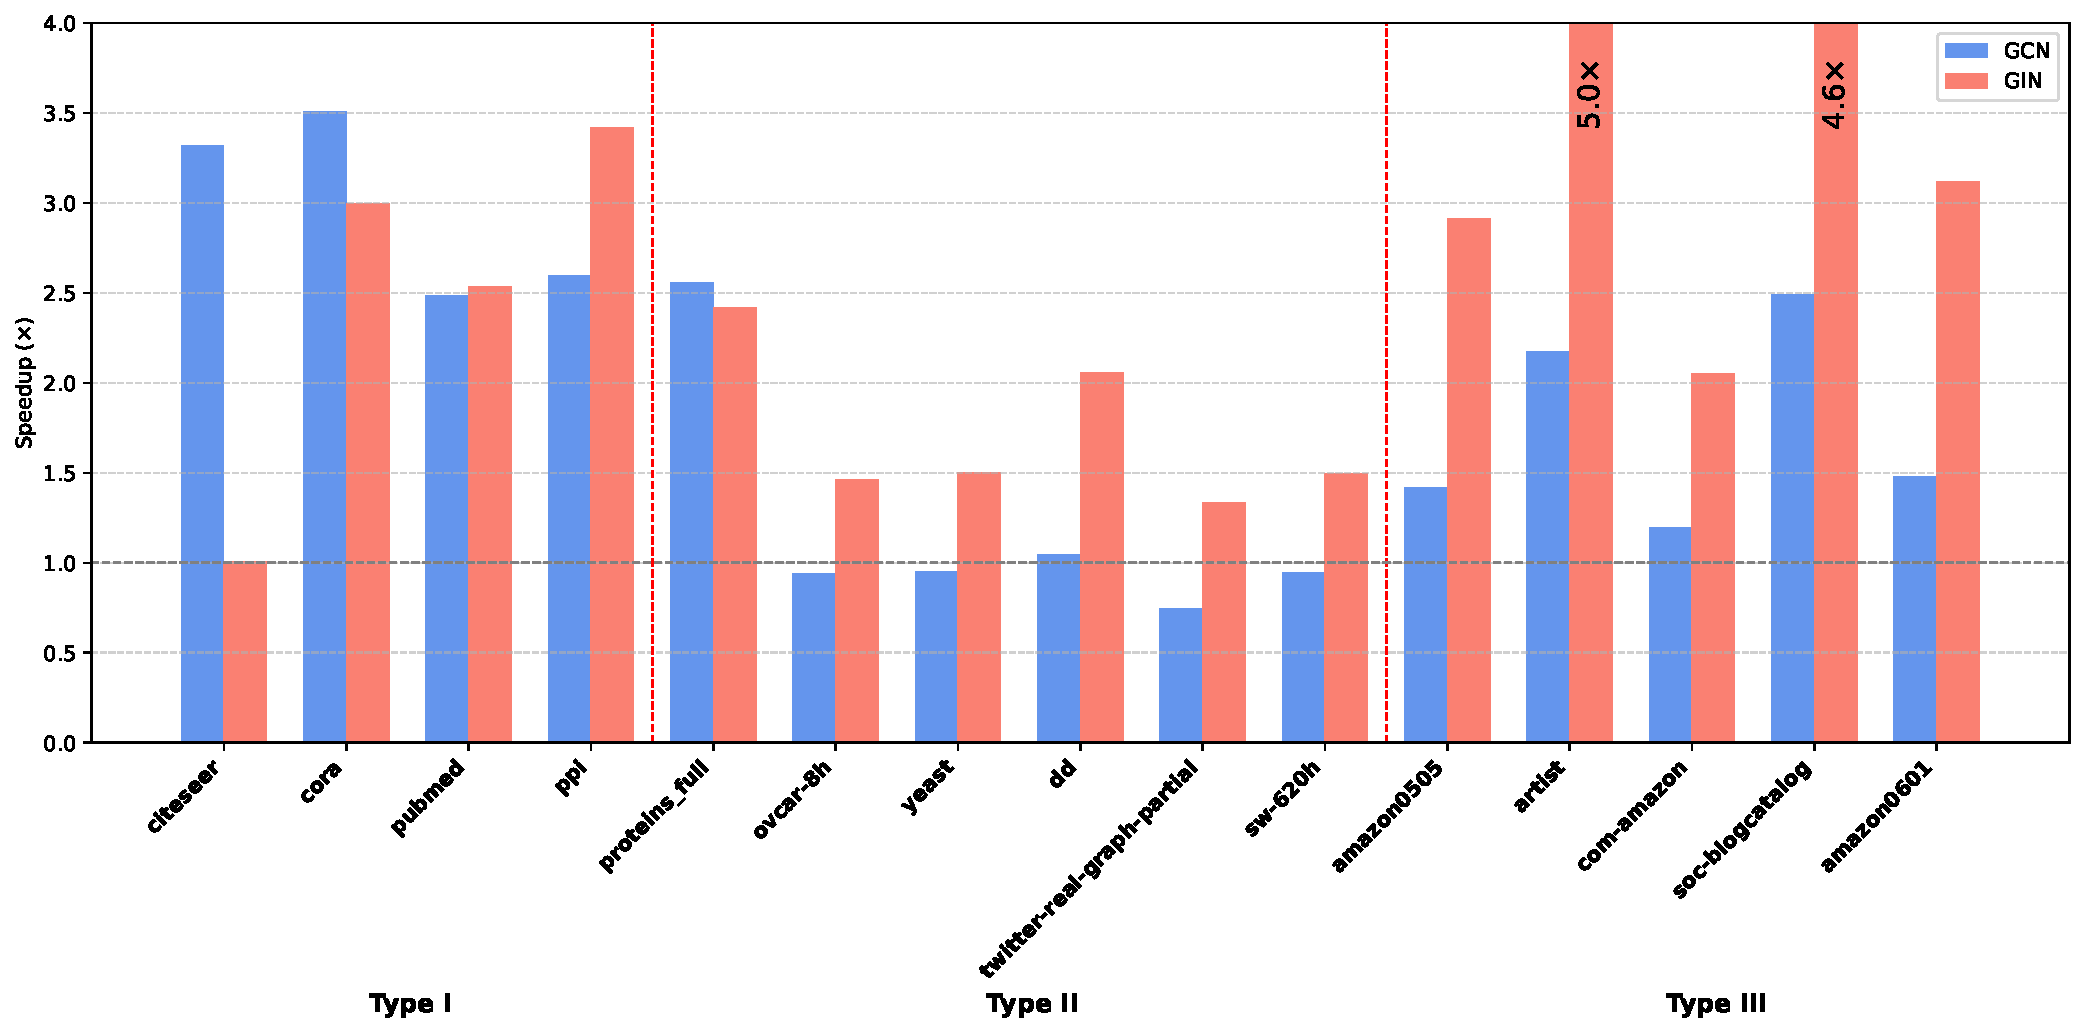
\includegraphics[width=0.9\linewidth]{images/pyg_train_cmp.pdf} 
    \caption{~\Mname{} 在 GCN 和 GIN 上相较于 PyG 的训练加速比 ($\times$)。}
    \label{fig: Speedup vs PyG Training}
    \setlength{\abovecaptionskip}{0.4cm} %增大caption和图像之间的距离    
    \setlength{\belowcaptionskip}{-0.4cm} %缩小caption和下方文字的距离
\end{figure}
\subsection{优化分析}
在这一节中,我们详细分析了第三章中设计的优化策略。
\begin{figure}[htbp]
    \centering
    \begin{subfigure}[b]{0.48\textwidth}
        \centering
        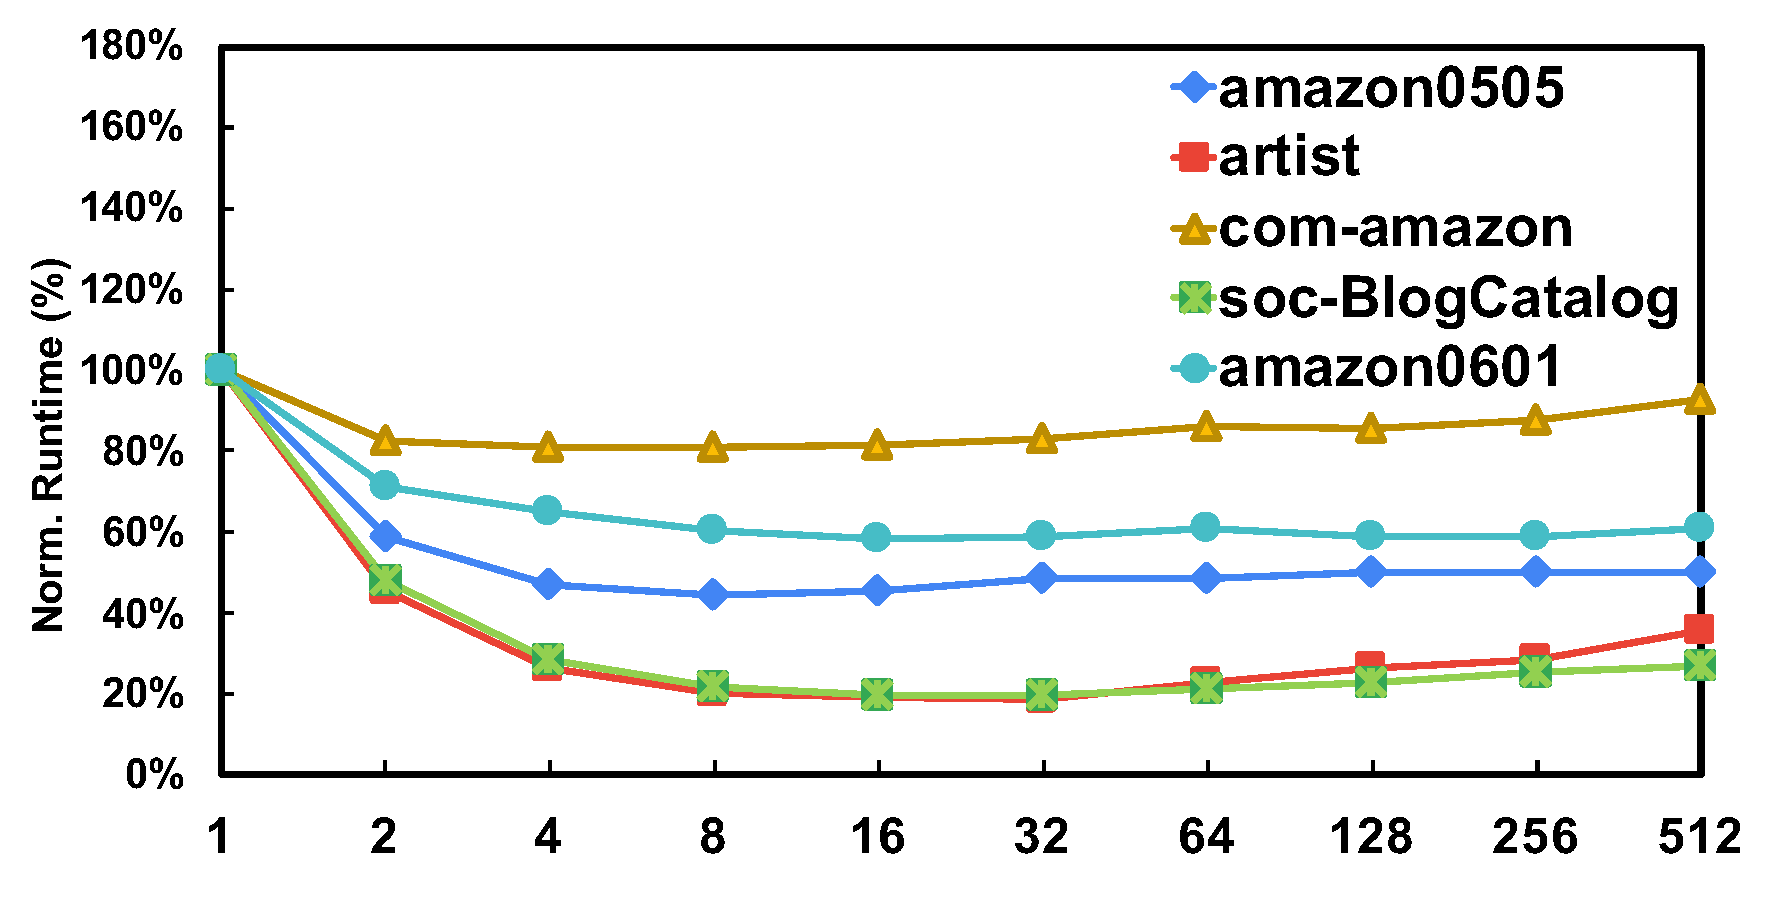
\includegraphics[width=\textwidth]{images/group-size-study.pdf}
        \caption{邻居分区大小对运行时间的影响}
        \label{fig:group-size-study}
    \end{subfigure}
    \hfill
    \begin{subfigure}[b]{0.48\textwidth}
        \centering
        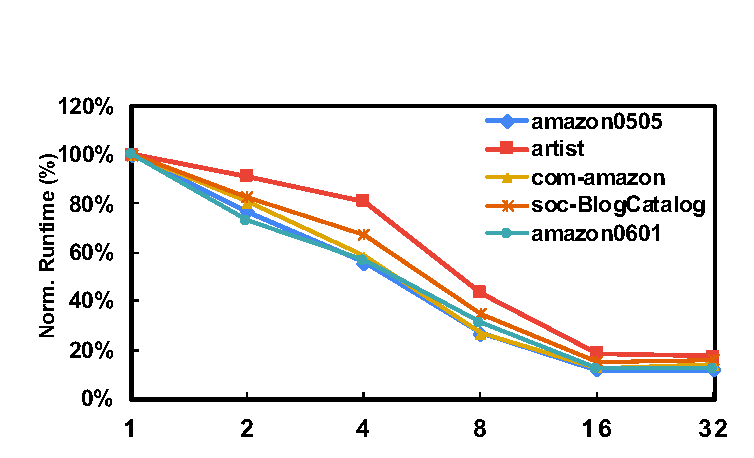
\includegraphics[width=\textwidth]{images/dimension-worker-1.pdf}
        \caption{维度工作线程数对运行时间的影响}
        \label{fig:dimension-worker}
    \end{subfigure}
    \caption{隐藏维度与延迟的关系}
    \label{fig:关于邻居分区和维度分区的研究}
\end{figure}
\subsubsection{邻居分区}
从图~\ref{fig:group-size-study}可以看出,邻居分区策略在优化线程并行效率方面起到了关键作用。随着邻居组大小的增加,~\Mname{}的运行时间最初呈下降趋势。这是因为更大的邻居组可以让每个线程处理更多的邻接节点,从而提高线程的计算饱和度,减少线程间的竞争与同步(如原子操作),同时提升缓存命中率,改善数据访问局部性。然而,当邻居组大小超过某个临界值(例如在 artist 数据集中为 32)后,线程的并行计算能力已达到上限,继续扩大邻居组会导致工作负载不均衡、部分线程空闲或等待,从而引发新的瓶颈,反而会增加总体运行延迟。
\subsubsection{维度分区}
如图~\ref{fig:dimension-worker} 所示,维度分区策略通过将节点嵌入特征向量的维度划分给不同线程来实现并行计算。当维度工作线程数量从 1 增加到 16 时,可以显著提升并行度和吞吐量,因为原本顺序执行的维度计算被拆分并发执行,显著缩短了关键路径。但进一步增加线程数量至 32 时,性能提升变得不明显。这是因为此时线程之间的并行性已基本饱和,系统资源(如寄存器、共享内存)竞争加剧,导致额外线程无法有效提升整体性能,还会引入额外的引入调度和同步开销。
\subsubsection{社区感知节点重编号}
我们通过对 GCN 和 GIN 在 III 型数据集上的分析,展示了节点重新编号的好处。如图~\ref{fig:reorder-speedup}所示,重新编号节点可以使 GCN 和 GIN 分别加速 1.14 倍和 1.09 倍。主要原因是我们的社区感知节点重新编号可以在 GNN 聚合过程中提高数据的空间和时间局部性。

为了量化这种局部性优势,我们提取了详细的 GPU 内核指标——DRAM内存读写字节数。CUDA 内核指标分析结果表明,节点重编号可以有效提升(GCN 平均减少 12.4\%,GIN 平均减少 9.3\%),因为重排序后提升了图的局部性,具有连续 ID 的节点更有可能共享已加载的节点嵌入。
\begin{figure}[htbp]
    \centering
    \begin{subfigure}[b]{0.48\textwidth}
        \centering
        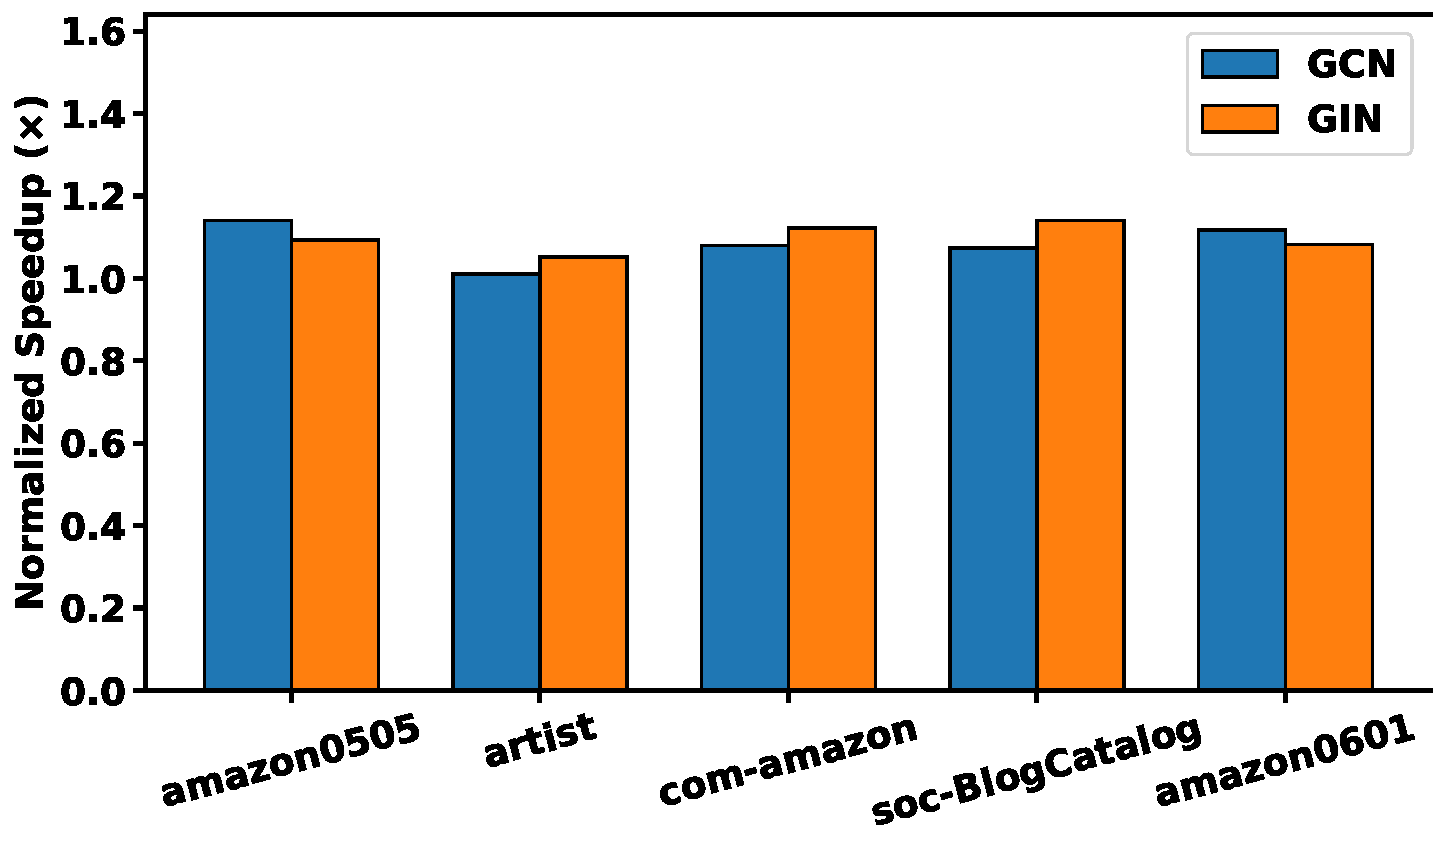
\includegraphics[width=\textwidth]{images/reorder_speedup.pdf}
        \caption{III 型图节点重编号前后的加速比}
        \label{fig:reorder-speedup}
    \end{subfigure}
    \hfill
    \begin{subfigure}[b]{0.48\textwidth}
        \centering
        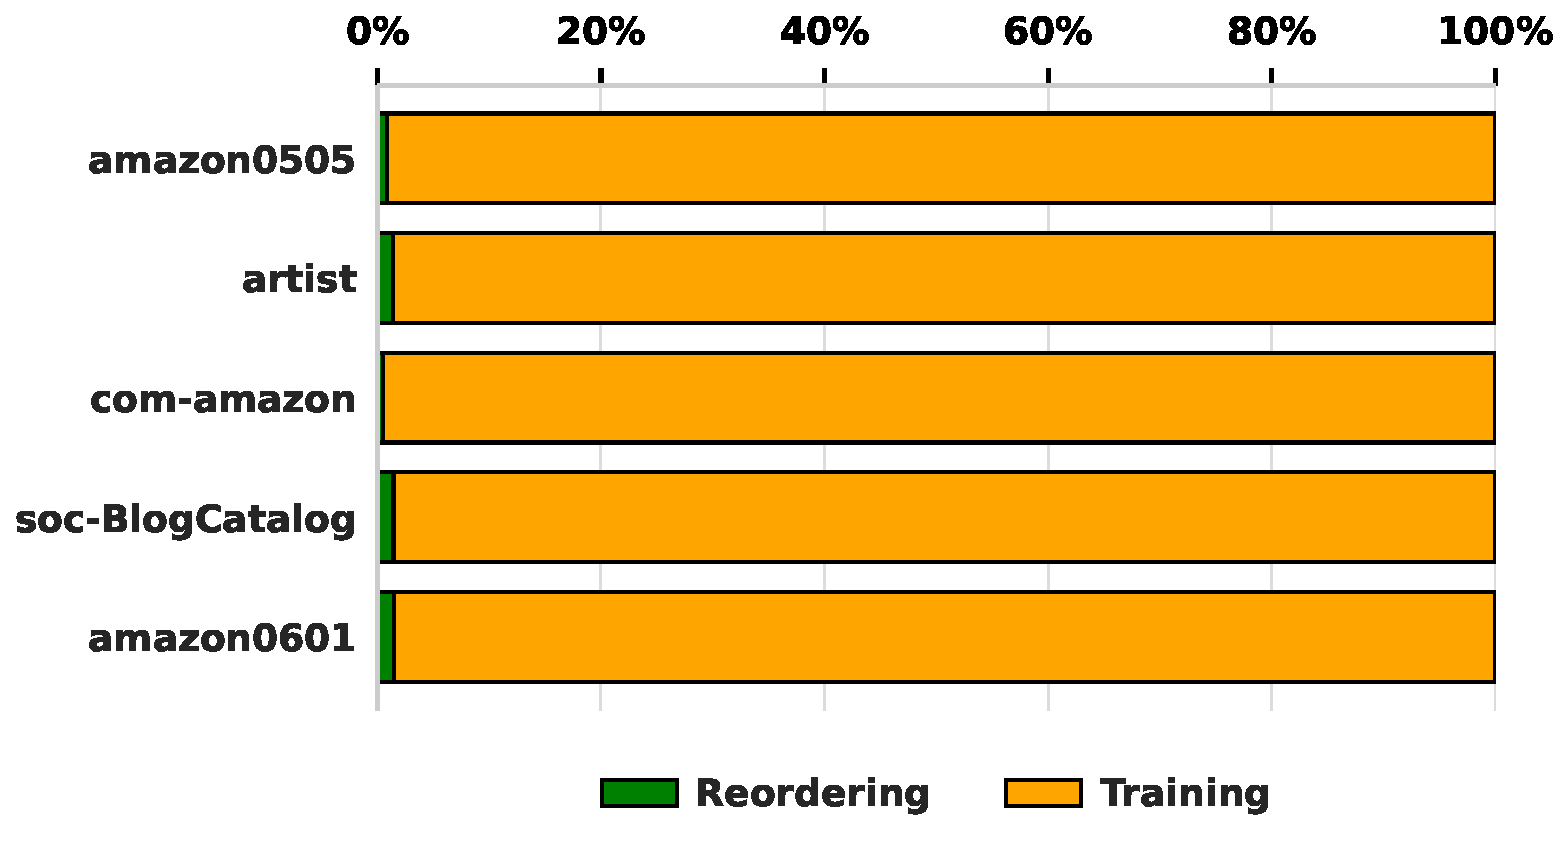
\includegraphics[width=\textwidth]{images/reorder_overhead.pdf}
        \caption{III 型图节点重编号的开销}
        \label{fig:reorder-overhead}
    \end{subfigure}
    \caption{节点重编号的加速比和开销}
    \label{fig:reorder}
\end{figure}


\subsection{额外研究}
~\label{sect: Additional Studies}
在这一节中,我们将对 GNN 的隐藏维度、~\Mname{} 预处理开销和\textbf{Decider}的参数选择等问题进行探讨。
\subsubsection{GNN的隐藏维度}
\begin{figure}[htbp]
    \centering
    \begin{subfigure}[b]{0.48\textwidth}
        \centering
        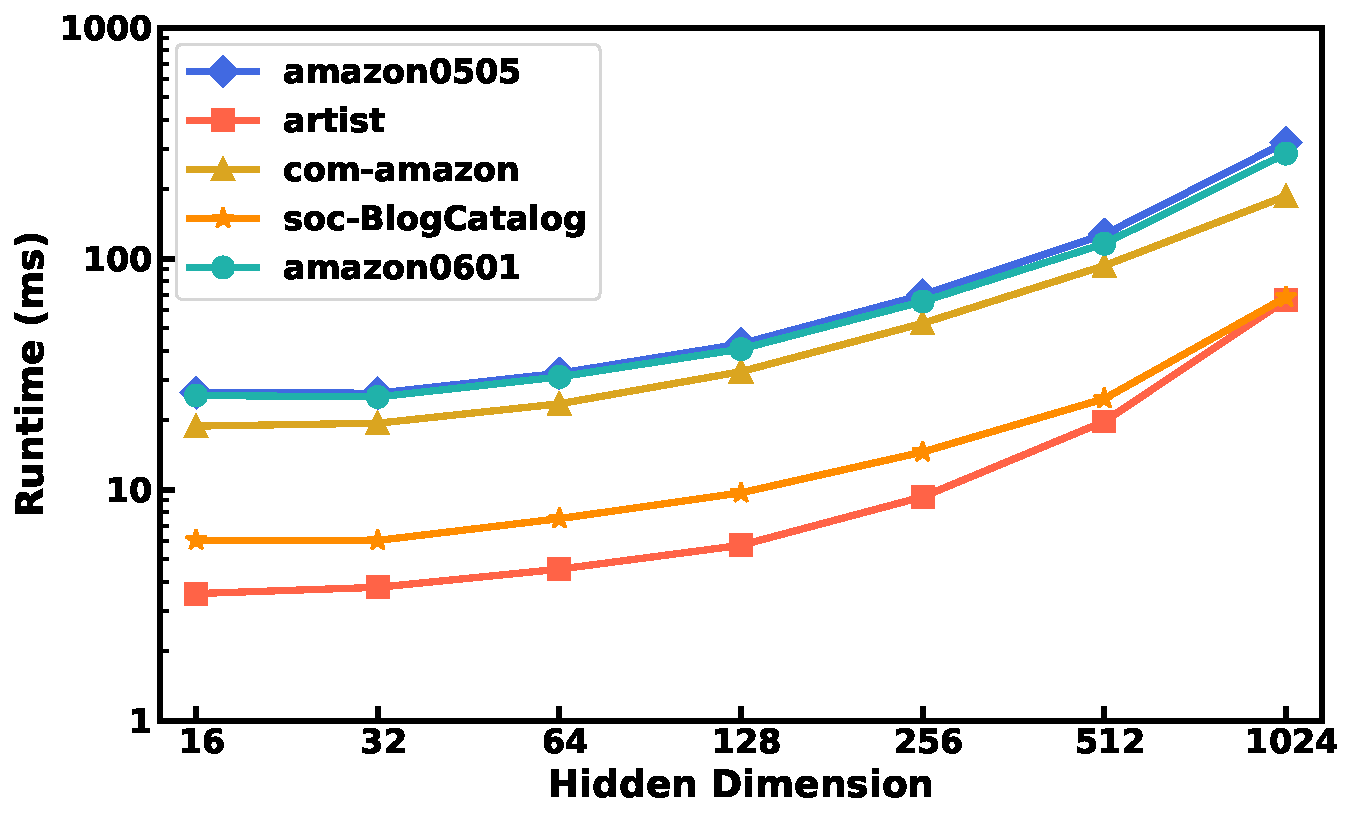
\includegraphics[width=\textwidth]{images/gcn_hidden_dim_runtime.pdf}
        \caption{GCN隐藏维度}
        \label{fig:subfig1}
    \end{subfigure}
    \hfill
    \begin{subfigure}[b]{0.48\textwidth}
        \centering
        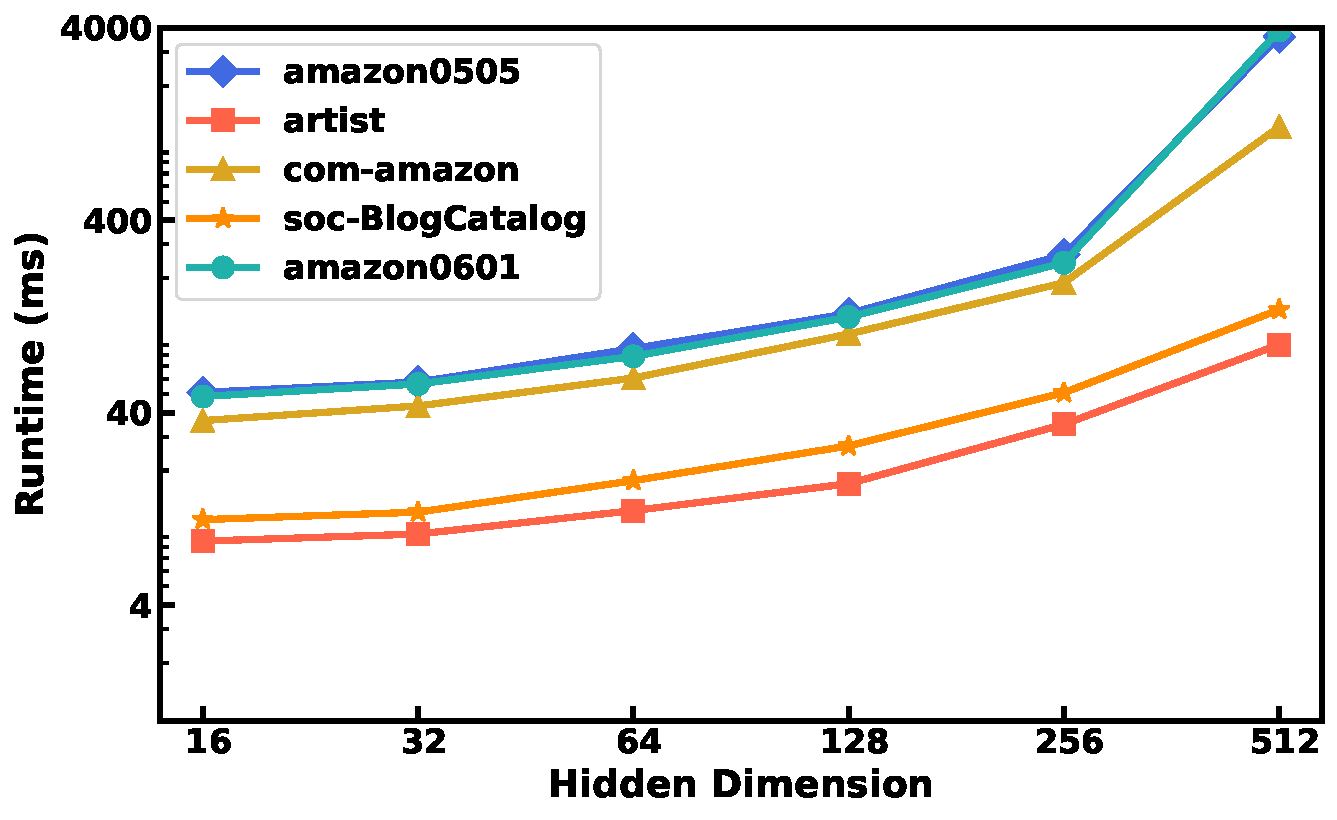
\includegraphics[width=\textwidth]{images/gin_hidden_dim_runtime.pdf}
        \caption{GIN隐藏维度}
        \label{fig:subfig2}
    \end{subfigure}
    \caption{隐藏维度与延迟的关系}
    \label{fig:Hidden Dimension}
\end{figure}
隐藏维度(hidden dimension)是 GNN 中用于表示节点特征的向量空间大小,它直接影响每一层神经网络的参数数量和计算复杂度。在本项实验中,我们重点分析了 GNN 架构中隐藏维度大小对两种主流模型——GCN 和 GIN——运行性能的影响。如图~\ref{fig:Hidden Dimension}所示,随着隐藏维度的增加,两种模型的运行时间均有所上升。这一趋势主要源于更大的隐藏维度带来了更多的计算和内存操作。在 GCN 中,聚合阶段会涉及更多的加法运算和数据移动操作,节点更新阶段的嵌入矩阵尺寸也随之扩大,从而增加了整体计算负担。

值得注意的是,GIN 的运行时间增长幅度远高于 GCN。这是因为 GIN 模型本身具有更深的网络结构(5 层),相比之下 GCN 仅为 2 层,导致隐藏维度带来的开销在 GIN 中呈线性甚至更高阶的叠加效应。此外,由于 ,GCN节点维度缩减(DGEMM)总是在聚合之前进行,这大大减少了聚合阶段的数据移动和线程同步开销。GIN 的聚合操作设计更复杂,在每一层的计算密度和内存访问强度都高于 GCN,因此在隐藏维度扩大时其性能退化更为明显。

\subsubsection{开销分析}
在 ~\Mname{}中,使用社区感知的节点重新编号来优化图的局部性,进而提升 GNN 的性能。尽管我们选用了轻量级的重新编号算法,但仍然需要在读取图后进行一次性预处理。为了评估这一开销对整体性能的影响,我们使用 GCN 模型对III 型图在训练阶段的性能开销进行了深入分析。III 型图的节点和边的数量,节点重编号的开销较大,同时结构高度不规则,容易从节点重编号中收益。图~\ref{fig:reorder-overhead}展示了训练过程中的重编号开销比例。可以看到,节点重新编号阶段的开销仅最高占训练时间的 1.52\%,平均仅占1.14\%。这一处理过程所带来的时间成本非常小,完全可以在训练或推理的运行时周期中进行摊销,从而避免对整体性能产生显著影响。

结合上一节的优化分析我们可以发现,这种一次性预处理策略不仅代价低,而且带来了显著的下游性能提升。通过对图结构的重组优化了图中节点的访问局部性,从而增强了后续计算过程中缓存命中率和数据传输效率。因此,社区感知的节点重新编号不仅在理论上具备可行性,在实践中也被验证为高效且轻量的优化方案。
\subsubsection{参数选择}

为了展示~\Mname{}中的轻量级分析模型\textbf{Decider}在内核参数选择中的有效性,我们在不同的数据集上进行了实验。我们选择了两个具有代表性的图数据集:\textit{amazon0505} 和 \textit{soc-BlogCatalog}。实验结果如图~\ref{fig: parameter selection}所示,\textbf{Decider}的参数选择策略能够为上述四种设置精确地找到最优的低延迟设计。这证明了我们的分析模型在辅助参数选择以优化 GNN 计算性能方面的有效性。

\begin{figure}[htbp] 
    \centering
    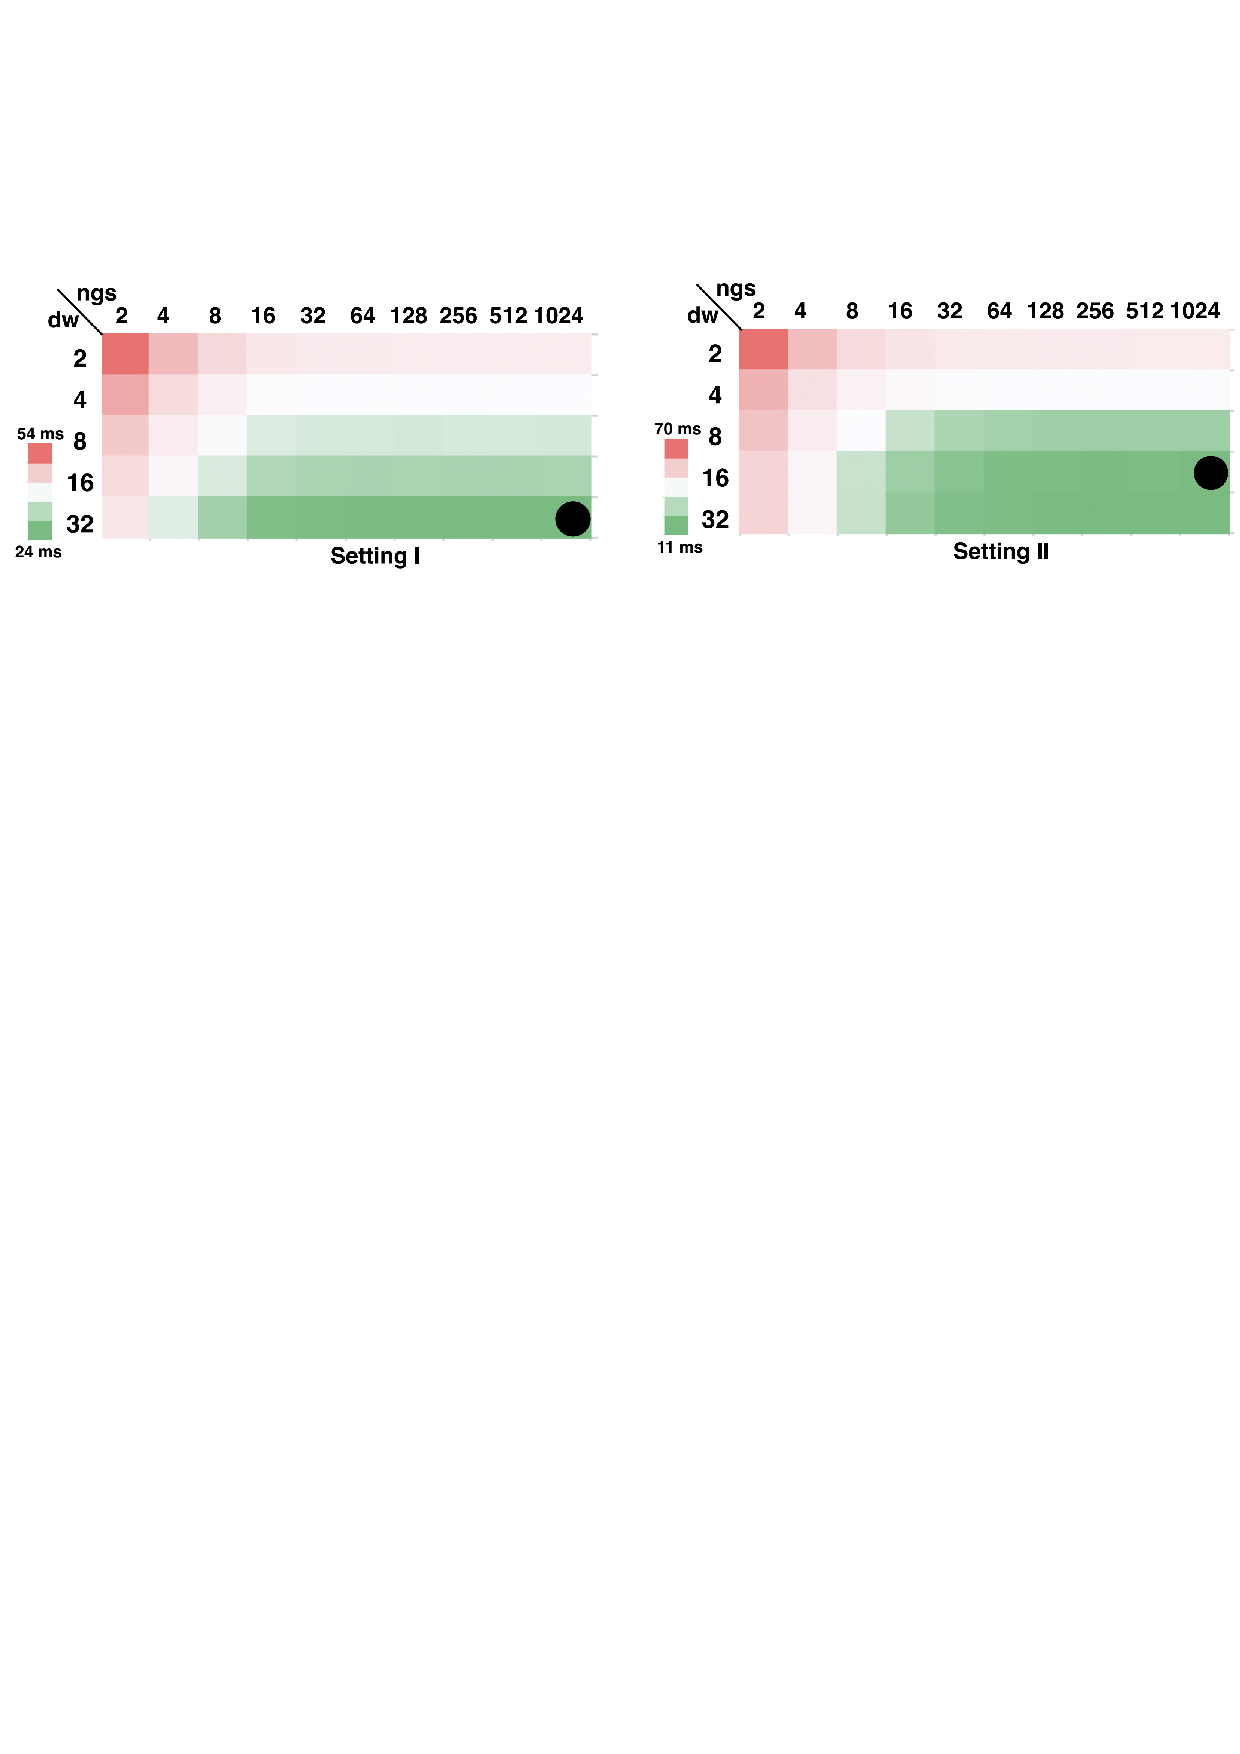
\includegraphics[width=0.9\linewidth]{images/paramer-2.pdf} 
    \caption{\textbf{Decider}的参数选择有效性验证,左侧为\textit{amazon0505}数据集,右侧为\textit{soc-BlogCatalog}数据集}
    \label{fig: parameter selection}
    \setlength{\abovecaptionskip}{0.4cm} %增大caption和图像之间的距离    
    \setlength{\belowcaptionskip}{-0.4cm} %缩小caption和下方文字的距离
\end{figure} 
\subsection{本章小结}
本章对~\Mname{}在多种GNN模型和三类图数据集上的推理与训练性能进行了系统评估。实验结果表明,\Mname{}在推理任务中相较于DGL平均加速可达$3.13\times$(GCN)和$1.35\times$(GIN),在训练任务中也实现了最高$2.00\times$的性能提升。这样的性能优势得益于\Mname{}基于图结构特征的任务划分策略和高效的内存优化机制,尤其在大规模、结构不规则的图上依然展现出显著效果。同时,我们还对~\Mname{}的预处理开销、参数选择等进行了深入分析,验证了其在实际应用中的有效性和通用性。


